\documentclass[a4paper]{article}

\usepackage[a4paper, inner=1.7cm, outer=2.7cm, top=2cm, bottom=2cm, bindingoffset=1.2cm]{geometry}
\usepackage[english]{babel}
\usepackage{graphicx}
	\graphicspath{ {images/} }
\usepackage{wrapfig}
\usepackage{paralist}
\usepackage{blindtext}
\usepackage{enumitem}
\usepackage{fancyhdr}
\usepackage{amsmath}
\usepackage[utf8]{inputenc}
\usepackage[toc,section=section]{glossaries}
\usepackage{enumitem}

\makenoidxglossaries
 
\newglossaryentry{java}
{
    name=Java,
    description={A general purpose object-oriented programming language}
}

\newglossaryentry{javafx}
{
    name=JavaFX,
    description={A graphical user interface library for Java}
}

\newglossaryentry{git}
{
    name=Git,
    description={An open sourece distributed version control software}
}

\newglossaryentry{github}
{
    name=GitHub,
    description={A web service that hosts git repositories for ease of use between developers}
}

\newglossaryentry{discord}
{
    name=Discord,
    description={A communication software hosted on the web used for scheduling, discussion and sharing of files}
}

\newglossaryentry{junit}
{
    name=Junit,
    description={A library in Java used for writing unit tests}
}

\newglossaryentry{latex}
{
    name=Latex,
    description={A textual interface for writing technical and scientific documents}
}

\newglossaryentry{javadoc}
{
    name=JavaDoc,
    description={A code documentation generator for Java}
}

\newglossaryentry{transcendentalfunction}
{
    name=Transcendental Function,
    description={"A function that does not satisfy any single-variable
polynomial equation whose coefficients are themselves roots of polynomials"}
}

\newglossaryentry{eclipse}
{
    name=Eclipse,
    description={A Java Integrated Development Environment}
}

\newglossaryentry{intellij}
{
    name=IntelliJ,
    description={A Java Integrated Development Environment}
}


\makeindex

\setlength{\parindent}{0pt}

\begin{document}


% TITLE PAGE CODE ------------------------------------
\title{\LARGE{\textbf{Team F - ETERNITY Calculator}}}
\author{
	Castonguay, Justin | Fakhr, Daniel | Hernandez, Jaime Andres \\ Thibault-Shea, Daniel |
	Yaghma, Ashkhan \\
}
\date{June 6, 2019}

\fancyhf{}

\clearpage\maketitle
\thispagestyle{empty} % Ensures no page numbering on title page
\pagebreak

\setcounter{page}{2} % Start counting on page 2
\fancyhf{}
\renewcommand{\headrulewidth}{2pt}
\renewcommand{\footrulewidth}{1pt}
\fancyhead[LE,RO]{\rightmark}
\tableofcontents
\pagebreak

\section{Team organization and collaboration patterns}

\subsection{Expectations}

The first thing on our order of business was to do a round table discussions to get everyone's expectations with regards to the team dynamics. The reason for this was so that we would all be on the same page.

\medskip

\textbf{Danny:}
\begin{compactitem}
\item Do mathematical research before coding any mathematical functions.
\item Be able to code in java and have decent technical knowledge 
\item Be willing to compromise ,or put matters to a vote, at times of conflict
\end{compactitem}
\textbf{Dan: }
\begin{compactitem}
\item The team should be a supportive place where member can develop - if someone doesn’t know something then the team should be able to teach them. We need to communicate actively and keep our peers in the loop.
\end{compactitem}
\textbf{Justin:}
\begin{compactitem}
\item I expect everyone to respect each other and have realistic expectations of one and other.
\item Everyone listen to each other and learn from each other.
\end{compactitem}
\textbf{Ashkan:}
\begin{compactitem}
\item It seems my level of knowledge is lower than the average of team. So I expect the team to bear with me, assign some simpler tasks to me in the beginning and support me to catch up as soon as possible.
\end{compactitem}
\textbf{Andres:}
\begin{compactitem}
\item I expect everyone to be respectful with each other
\item I expect everyone to communicate with each other openly
\item I expect everyone to be able to communicate if they will not be able to finish a part on time in a timely manner, so adjustments can be made before the deadline with minimal stress
\item I expect the work to be spread fairly
\item I expect the work to be spread out considering everyone’s skill sets and what they would like to work on themselves
\end{compactitem}

\textbf{Expectations Agreed on:}
\begin{compactitem}
\item The team should be a supportive place where member can develop - if someone doesn’t know something then the team should be able to teach them. We need to communicate actively and keep our peers in the loop.
\item Respect one another
vLearn from each other
\item Listen 
\item Communicate openly and constructively
\item All tasks must be completed before the given deadline
\item If work will not be finished it MUST be communicated in a timely manner so the team can support and readjust our strategy to deliver our work on time
\item Team outings after milestones on a budget
\item Distribute work fairly, evenly, and considering each member’s skill level.
\end{compactitem}
\bigskip

This document hereby confirms that all group members listed agree to follow through with these expectations throughout the timespan of this whole project. 


\begin{center}
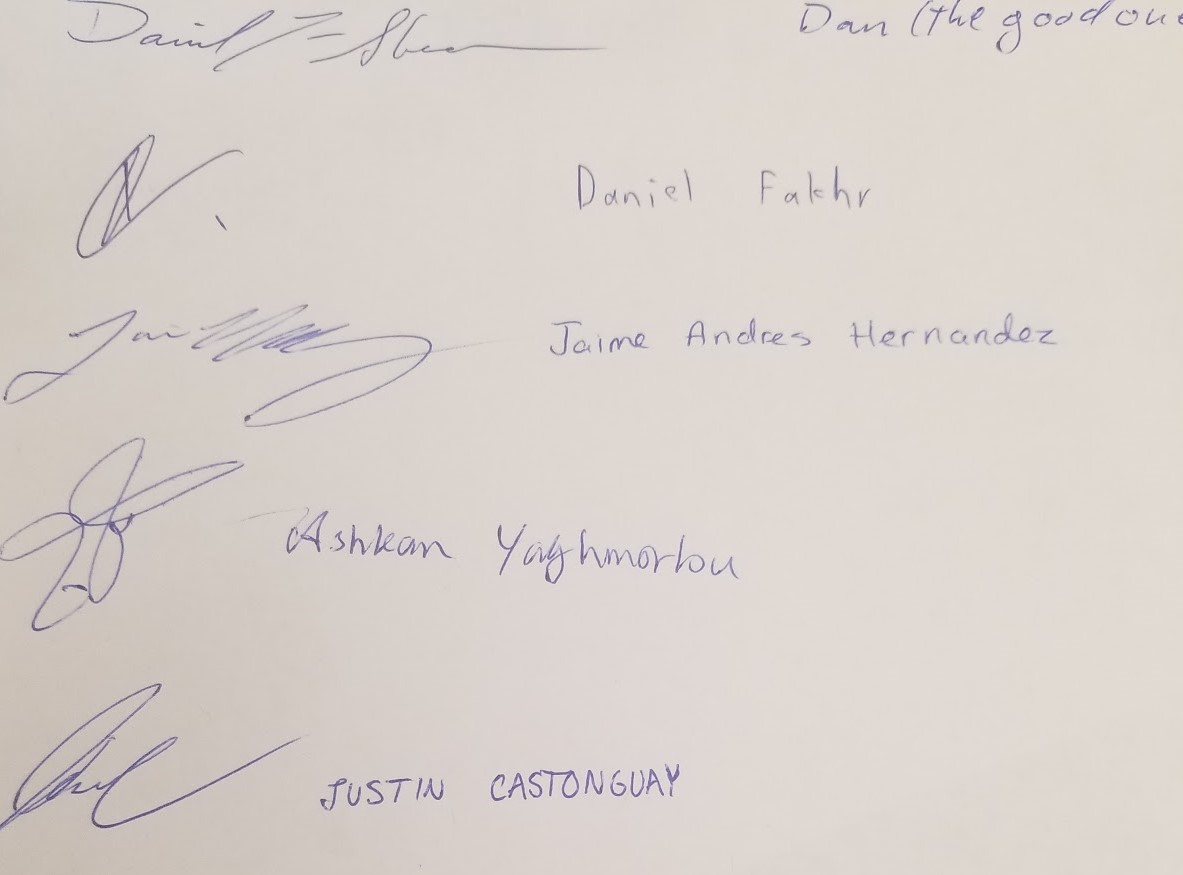
\includegraphics[width=0.4\textwidth]{ExpectationSignatures.jpg}
\end{center}

\subsection{Meeting Schedule}

We agreed to meet at least once a week for 2 hours. We are also in constant contact on Discord and we all keep apprised of recent pushes to the Git repository to stay up to date with the advancement of the code base and the accompanying documents. Detailed meeting minutes are posted to the Git repository after every meeting by the designated secretary for that meeting. We are also using Google Docs to collaboratively work on draft documentation, which can then be used to create our final documentation with the correct formatting.

\subsection{Our Strategy}

In order to develop a working software calculator prototype in the coming weeks, our team has come up with a development strategy to be prepared for challenges that we may face. This strategy must take into account a plan for writing requirements for features implemented, the technologies selected to develop the calculator, ideas of algorithms for numerical computation of selected functions, and tasks to be allocated to each team member based each of our strengths. With a well advised plan of action, we are much more likely to collaborate efficiently as a team and ultimately meet the deadline of the project. 

\subsection{Choice of technology}

Our team needed to select technologies to meet our software needs while also complementing the team members’ development expertise. The necessary technologies included:
\medskip
\begin{compactitem}
\item main programming language with unit testing libraries, a code documentation interface and a graphical user interface library
\item communication tools
\item version control software
\end{compactitem}
\medskip
For our primary programming language we decided to pick the language in which all of our team members had experience writing code in, Java. This allowed each team member to jump right into coding when the time came since no one was blocked having to learn a new language. Java is also advantageous since it has many libraries that we would be able to use for unit testing (Junit), GUI development (JavaFX) and code documentation (Javadoc). Additionally, its object-oriented design fit with how we envisioned designing our calculator program. \\

In order to coordinate with each other outside of regular meeting hours, we decided to use Discord as our communication tool. Discord can be accessed on almost any device, is very reliable and is easy to use. It also allowed us to create different chat channels for different subjects in order to keep our discussions on topic. For example, one channel could be for scheduling and one could be for brainstorming ideas about algorithms. \\

We decided to choose git as our version control software since it is simple enough to use, it has tons of documentation to support our needs and some of our team had already used it. Furthermore, they would allow us to work on the same files at different times and easily keep track of changes made to any of the files. 

\subsection{Task assignment}

During the second team meeting we went over the requirements for deliverable 1 and made a list of all of the things that needed to get done. We quickly saw that this was a significant amount of work and that there were some dependencies between the tasks (ex. do interviews before use cases). We divided the tasks into 3 categories: 1) Information gathering, 2) Consolidation/Report, 3) Coding and prototyping. A cursory evaluation of the workload vs. the deadline showed that we could not possibly deliver all of these tasks on time. Rather than cut out the early-stage prototyping entirely, we decided on making a priority matrix of our tasks with the simple rule that higher priority tasks should be completed before an individual started work on the lower priority ones. \\

We reasoned that the top priority items were those on the critical path of deliverable 1. We all had a good idea of what a calculator should be but we also knew better than to make a product for the developers. Consequently, we absolutely needed the information from the interviews as soon as possible so that we could align our efforts with what the calculator's potential users wanted. This step was so critical and urgent that we put 4 people on it with highest priority. \\

We then consolidated and paraphrased the interview data. We were surprised at just how much information we got from 5 interviewees. Firstly, we extracted the key features each user wanted. Secondly, we distilled down each interview into the key themes that were important for that interviewee. Thirdly, we were able to classify our interviewees based on their expected usage of the calculator (basic use, mathematical use). Lastly, we looked for commonality across the different wants of the interviewees and obtained what we think is a much better approximation of what the market wants from a calculator. \\

One team member was tasked with coming up with an outline of our testing strategy. We decided that since the users all seemed to value accuracy of the mathematical function on the calculator then a test-driven approach to development would be appropriated. \\

Another person was tasked with researching the algorithms needed for the implementation of the non-trivial calculator functions. Some functions had multiple algorithms that varied in complexity. For this first iteration, it was decided that simplicity should be the key criteria in the choice of algorithm since the deadline was so tight. We all agreed that we could reevaluate this strategy for the next iteration. \\

The very last priority was the implementation of the mathematical functions. Some team members were eager to start coding but we decided that it would be a much better idea to focus on the requirements gathering at this stage of development. Consequently, only a very rough implementation of some of these functions appear as code. \\

\begin{table}[ht]
\centering
\caption{Task Priority Matrix}
\begin{tabular}{|l|l|l|l|}
\hline
\textbf{Name}&\textbf{Priority 1}  &\textbf{Priority 2}  &\textbf{Priority 3}  \\ \hline
 Ashkhan&Interviews/personas  &Testing strategy (TDD)  &$a^x$, $10^x$  \\ \hline
 Daniel F.&Interviews/personas  &Algorithm research  &$x^y$, $\sqrt[n]{x}$  \\ \hline
 Daniel T.&Coordinate activities  &Use case diagram/desc  &$e^x$  \\ \hline
 Jaime&Interviews/personas  &Interview summary  &$cos(x)$, $sin(x)$  \\ \hline
 Justin&Interviews  &Strategy  &$ln(x)$  \\ \hline
\end{tabular}
\end{table}

\subsection{Testing strategy}

For testing purposes, we decided to use Junit to write all of our unit tests. These tests would verify the functionality of our different mathematical functions. We would need to think of and write up as many test cases as possible for different scenarios (negative numbers, large and small numbers, invalid input, etc) in order to cover all potential issues. \\

Test coverage is incredibly important in the early stages of a software project. Early and thorough testing reduces the risk of having an insurmountable amount of bugs later on. Taking this into consideration, we decided to employ a Test Driven Development strategy in which we would write unit tests before the functions were complete and imposed a rule that all valid tests must pass before any team member makes a push to our master branch. This would ensure that whenever anyone pulled from the master branch, they would not have to waste time fixing someone's bugs to work on their own task. \\

We all agree that testing each other's code is of paramount importance to the project. To not do so would lead to colossal wastes of time in tracking down myriad bugs. We made the following testing matrix which will ensure that there are no conflicts of interest in the testing. The arrow indicates who can test who - no arrow means you cannot test that person's code.

\begin{figure}[!h]
\caption{Testing matrix}
\centering
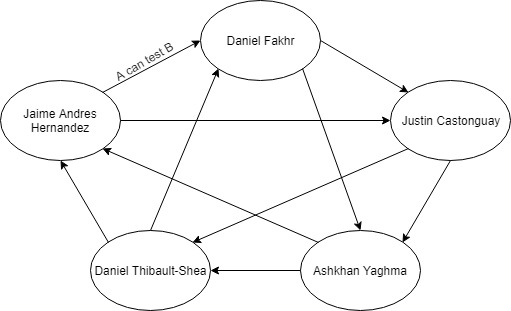
\includegraphics[width=0.75\textwidth]{TestingMatrix}
\end{figure}

The source code peer review was organized such a way that no pair of people review each others code. \\

The code review was done in the similar order :

\medskip
\textit{Jaime Andres Hernandez $\rightarrow$ Daniel Fakhr $\rightarrow$ Justin Castonguay $\rightarrow$ Ashkan Yaghma $\rightarrow$ Daniel Thibult-Shea $\rightarrow$ Jaime andres Hernandez.}
\medskip

The following table summarize some of the code reviews that were undertaken and the associated comments provided to the reviewees.


\begin{table}[]
\begin{tabular}{|l|l|l|}
\hline
Reviewer                                                            & Reviewee                                                         & Comments                                                                                                                                                                                                                                                                    \\ \hline
\begin{tabular}[c]{@{}l@{}}Jaime\\ \\ Andres Hernandez\end{tabular} & Daniel Fakhr                                                     & \begin{tabular}[c]{@{}l@{}}-Try to follow Proper formatting\\ (some of your code is not properly indented)\\ -Try to comment more, some functions are missing comments.\\ \\ -Use JavaDoc comments so we can auto-generate docs\end{tabular}                                \\ \hline
Daniel Fakhr                                                        & Justing Castonguay                                               & \begin{tabular}[c]{@{}l@{}}-Use more comments. Some of your comments are uncommented\\ -Test your functions. Some of them don't work as they should \\ -Use "throws Exception" in the method declaration when not \\ catching the Exception within the method.\end{tabular} \\ \hline
Justing Castonguay                                                  & Ashkan Yaghma                                                    & \begin{tabular}[c]{@{}l@{}}-Format your code better\\ -Use better variable names\end{tabular}                                                                                                                                                                               \\ \hline
Ashkan Yaghma                                                       & Daniel Thibault-Shea                                             & \begin{tabular}[c]{@{}l@{}}-Don't leave commented code.\\ -Comment your functions.\end{tabular}                                                                                                                                                                             \\ \hline
Daniel Thibault-Shea                                                & \begin{tabular}[c]{@{}l@{}}Jaime\\ Andres Hernandez\end{tabular} & \begin{tabular}[c]{@{}l@{}}-Write JavaDoc comments (including comments for constants)\\ -Elaborate more in your comments \\ -Try to make your code more efficient\end{tabular}                                                                                              \\ \hline
\end{tabular}
\end{table}



\pagebreak

\section{Requirements Gathering}

In order to create software requirements, our team got together to brainstorm ideas for what features the calculator would have and how to implement them. We made sure our features were realistic, keeping in mind the time constraint of the project and the development experience of the team. Once we had a base for how we thought our calculator could be developed, we decided to conduct interviews on potential users to find out what features everyday users of calculators actually valued and if our initial ideas complemented these. \\

From the answers from our interviewees, we created user personas that had concrete problems and tasks that needed to be completed and that our software would solve. The user personas along with our initial discussions would then inform what different use cases might be for our calculator. The use cases were put into a standard use case diagram so that the high-level design of the calculator could be understood at a glance. Each use case was then expanded in a summary use case description.

\subsection{Common interviewee points summarized}

\textbf{\ \ \ \  Sarah}

\underline{HR Student}

\begin{compactitem}
\item inputting full eqn like she memorized
\item physical calculator 
\item simple calculator
\item prefers physical calculator but uses others
\item functions in the book
\item downloadable functions or packages
\item cares about precision and the right answer
\item doesn’t care about aesthetics
\item hot keys for common functions
\end{compactitem}
\bigskip

\textbf{Victoria  Benlala}

\underline{Entrepreneur, Spa Owner}

\begin{compactitem}
\item Button to calculate the taxes (simple programmable functions)
\item phyiscal calculatior first doesn’t mind others
\item doesn’t use complicated functions
\item simplicity and soft buttons. Would like a more portable version.
\item mapping numbers to number keys on computer. Being able to have hot keys or set them up himself with the functions he or she is given
\end{compactitem}
\bigskip

\textbf{Kevin}

\underline{Engineering student}

\begin{compactitem}
\item Would like to be able to access functions easily for engineering 
\item Comfortable with both software and hardware but prefers hardware
\item He wants shortcuts
\item Wants basic functions also
\item Wants to use computer keyboard and not mouse pointer
\item Portable and key mappable
\item Use symbols that are already commonly found on calculator on the cpu keyboard also 
\item Include a shortcut quit key
\item Hot keys (like S for sin, T for Tan, etc.)
\item Recommends skins for calculator
\item Would like downloadable packages for functions to customize calculator
\end{compactitem}
\bigskip

\textbf{Tarek}

\underline{Electrical engineering student}

\begin{compactitem}
\item accuracy, speed, and comfort
\item basic essential functions
\item he would like it to be able to plot graphs 
\item he would like to transfer his work from calculator to mobile
\item prefers physical but he uses other for quick calculations
\item wants calculator easy to hold
\item would like it to be cheap even if it’s customizable
\end{compactitem}
\bigskip

\textbf{Arash}

\underline{Avionics Engineering Student}

\begin{compactitem}
\item specific buttons for each function
\item prefers an app 
\item He would assign each function to a specific button
\end{compactitem}


\subsection{Common Ideas}
\begin{itemize}
\item Simplicity 
\item Physical calculators $\rightarrow$ GUI could look like physical calculator
\item Hot keys 
\item Simple functions (plus, minus, etc.) 
\item Portability 
\item Customizable (physical and software wise)  download functions 
\end{itemize}

\subsection{Interview Data Summary}

Looking through all the interviews we were able to pick up on some important points that we chose to consider when creating our use case diagrams and to move forth with our project. We interviewed a Human Resource, Mechanical Engineering, Electrical Engineering, and Avionics Engineering student. We also interviewed an Entrepreneur/Spa Owner to gather our data. Each individual had very different needs specifying what kinds of functions they would like to see on their ideal calculator. For example, Engineers wanted integration functions, while an entrepreneur wanted percentages or tax calculating functions. \\

What they all had in common though was the want for simple operations (like addition, subtraction, etc.). They all also wanted simplicity in terms of the calculator's look, how easy it would be to access the functions they wanted to use, understand what they are, and it’s portability. The majority also wanted a reliable calculator in terms of precision and accuracy. They all preferred physical calculators over software calculators (like those you would find on a computer as an extra tool application). They all liked the idea of mapping keys on a computer keyboard to their desired functions to make the calculating experience more personalized and simple to them. They all had different ways they wanted to customize their calculator, which included personalizing it physically and software-wise. The important point though was that customizability was what they valued commonly amongst each other. \\

Based on the research we made from the stakeholders we interviewed, the calculator will need to be \textbf{simple}, \textbf{customizable}, and \textbf{reliable}.

\subsection{Use cases}

With the initial requirements gathering step mostly completed, we were now able to 

\begin{center}
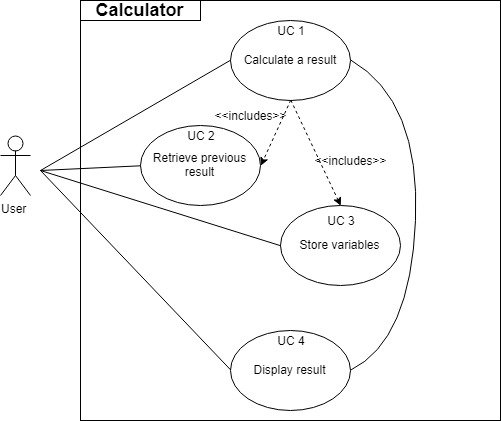
\includegraphics[width=0.5\textwidth]{UseCaseDiagram.jpg}
\end{center}

\section{Prototyping}

\subsection{Source code overview}

This iteration was mostly marked by requirements gathering mainly through the interview process. A limited amount of research was done into evaluating different algorithms for implementing of some functions. \\

While that was ongoing, we thought that we needed something concrete to present at this stage. While nothing look even remotely like a calculator at this stage, several function were implemented satisfactorily. \\

For example, $ln(x)$, $sin(x)$, $e^x$, and $\sqrt[n]{x}$ were implemented with some measure of success. Choices were made to used the simplest algorithm at this stage and to only test over a certain range of inputs. The full implementation will be done for the next iteration. \\

Following the interviews with the engineering students, we decided on implementing some extra functionality such as $x!$, binomial coefficient, etc. to better satisfy this class of users's needs. We were able to justify their inclusion at this early stage in part due to their relatively simple implementations. \\

There are still an immense amount of implementation details that the team needs to agree on at this stage. The interview process gave us so many ideas and potential requirements/features that we have not had enough time to debate on. We reserve the resolution of these issues for the next iteration. At this stage, it is exciting to see how the product is taking shape. With every meeting we feel we are getting tangibly closer to the final version of the product. We know that we will have some hard decisions to make very soon and that there may be some slight head butting. Regardless, we are all keen on compromising and getting a good product out the door.

\subsection{Algorithms evaluation}

Based on our experience and with the information gleaned from the interview, we decided to implement at least the following transcendental functions: $x^y$, $e^x$, $sin(x)$ and $cos(x)$, $tan(x)$, $ln(x)$ and $sqrt(x)$. Currently, optional functions are $arcsin(x)$, $arccos(x)$, $arctan(x)$. In order to develop solutions for our calculator without help from Java’s math library, we would have to do research on numerical methods to compute these functions. We would have to find the sites with mathematical references such as Wolfram-Alpha, Wikipedia and YouTube in order to find solutions that would be feasible for us. \\

A few of these functions $(sin(x)$, $cos(x)$, $tan(x)$, $e^x$, and the $arc*(x)$ functions could be approximated relatively easily by Taylor polynomials. Series lend themselves naturally to iterative methods (ie. simple 'for' loop) so that is what these algorithms are.
\bigskip

For example, here is the algorithm for $e^x$:

\begin{center}
\begin{tabular}{l}
$result\leftarrow 0$ \\

$precision\leftarrow p$ (arbitraty precision integer) \\

\medskip
$iterator\leftarrow 0$ \\

\textbf{while} $iterator < precision$ \textbf{do} \\

$\;\;\;result\leftarrow result + \frac{x^i}{i!}$ \\

\medskip
$\;\;\;i\leftarrow i + 1$ \\

\textbf{return} $result$ \\ \\

\end{tabular}
\end{center}

This algorithm does not pass test for a wide range of values of $e^x$. Currently, we are debugging this. This is an extremely simple algorithm compared to the other but they mostly take this form. The complexity of this particular algorithm is constant, however, it calls the $x^i$ function which we have implemented hamfistedly as $x$ multiplied by itself $i$ times. We intend to optimize the power function in later iteration to take advantage of the many optimizations possible (ie. bitshifting, etc.). \\

The algorithm for $ln(x)$ is:

\begin{center}
\begin{tabular}{l}
{\textbf{if}} $result\leq 0$ \\
$\;\;\; return$ {\textbf{error}} \medskip \\ 

$precision\leftarrow p$ (arbitraty precision integer) \\

\medskip
$iterator\leftarrow 0$ \\

\textbf{while} $iterator < precision$ \textbf{do} \\

$\;\;\;result\leftarrow result + \frac{1}{(2i+1)} * \frac{(x-1)}{(x+1)}^{(2i+1)}$ \\

\medskip
$\;\;\;i\leftarrow i + 1$ \\

\textbf{return} $(2*result)$

\end{tabular}
\end{center}

The $ln(x)$ algorithm is of a similar vein as $e^x$ and of a similar complexity. Tests have been successful up to about x = 870. We are still debugging this. We think it has something to do with our algorithms being centered around 0 and the solution becoming less and less precise as we increase or decrease x away from 0. We will definitely have this sorted out for iteration 2.

\subsection{Exclusions}

Between the requirements gathering and the work we have already done on the prototype calculator we feel we are in a much better position to evaluate what features and functionality we can currently commit to (see task matrix) and which we must exclude. The following features were discussed and rejected for reasons that are documented in brief in the following table.
\bigskip

\begin{tabular}[!h]{|p{3.5cm} | p{10cm}|}
\hline 
\textbf{Feature} & \textbf{Reason} \\ 
\hline 
Distributed on web & No one has web skills. Everyone knows Java. \\ 
\hline
User customizations & We are not able to determine the workload that this represents since we are not far in the development of the calculator - TBD.  \\ 
\hline
Mobile & Team does not have the skills to do that. \\
\hline
Hyperbolic functions & We don't even know what they are. The engineering interviewees never really used them except for \"that one class\". We don't think they are worth the effort. \\
\hline
Distributed on web & No one has web skills. Everyone knows Java. \\ 
\hline
Animations & No one has any skills with that. This will be the first GUI for some of us. \\ 
\hline
\end{tabular} 
\bigskip

The factor that most limits our willingness to undertake new functionality and features is the lack of skills found within the team. We all have the best intentions and want to provide a fully featured calculator but we had to draw the line somewhere. Currently, we are managing this by concentrating on the deliverable and focusing on the key features that the interviewees brought up. \\

\pagebreak
\section{Appendices}

\subsection{Appendix A - Interview Questionnaire}

\vspace{1in}
{\centering{\Huge Suggested Interview Questions}}
{\centering{\LARGE ETERNITY Calculator - Team F}}

\begin{center}Name: \line(1,0){275} \end{center}
\begin{center}Occupation: \line(1,0){270} \end{center}

{\centering{\textbf{\Large Suggested Interview Questions}}}

\begin{enumerate}
\item What do you use a calculator for?
\item What would you like your calculator to do? Or what is the ideal calculator for you?
\item What kinds of calculators have you used? (physical, apps, online, etc.). Hardware or Software? 
\item What functions do you use most often? Which ones do you use the least?
\item What features did you like most about your calculator. What do you not like about your calculator?
\item Is the aesthetics of your calculator important? What matters most (shape, color,  personalized themes, etc.)?
\item If you’re using a keyboard, how would you map the keys to functions, numbers, etc. ergonomics?
\end{enumerate}

\pagebreak

\subsection{Appendix B - Interview transcripts}

\subsubsection*{Interview Q\&A - 1st year HR student}
\textbf{What do you use a calculator for?}
\begin{itemize}
\itemsep0em 
\item Almost exclusively for her accounting and finance classes
\item Most of her usage of the calculator is for simple lightweight math used in accounting and finance.
\item She does not use it extensively, mostly for exams and homework.
\end{itemize}

\textbf{What would you like your calculator to do? Or what is the ideal calculator for you?}
\begin{itemize}
\itemsep0em 
\item She likes her calculator to be simple
\item Prefers a calculator that has its function symbols identical to the ones in the books
\item She would like her calculator to display the answers in a human readable form (5x7 Matrix numeric representation), and not the digital form (7-segment numeric representation)
\item In the future she would like to see a calculator network system, similar to that of the iclicker, where the professor would give you a password, which after inputting it into the calculator, downloads a custom function from the professor's base station, or unlocks/locks some of the pre programmed functions in the calculator.
\end{itemize}

\textbf{What kinds of calculators have you used? (physical, apps, online, etc.). Hardware or Software?}
\begin{itemize}
\itemsep0em 
\item Uses both a physical calculator as well as a calculator app on her phone.
\item Mainly uses the calculator application because it’s always available.
\item Prefers the physical calculator since she enjoys the tactile feel of the buttons and because phones are not allowed during exam time.
\end{itemize}

\textbf{What functions do you use most often? Which ones do you use the least?}
\begin{itemize}
\itemsep0em 
\item Most of the time she uses functions such as: addition, subtraction, delete (backspace) , $10^x$, Ans function for retrieving the previous answer , exponential and square root.
\item Rarely, if ever, uses logarithms or any of the trigonometric functions.
\end{itemize}

\textbf{What features did you like most about your calculator. What do you not like about your calculator?}
\begin{itemize}
\itemsep0em 
\item She feels indifferent about what she likes in her calculator. All she cares about is that the calculator gives the right answer.
\item The only thing she does not like about her calculator is that it displays numbers in a digital format (7 segment numeric representation)
\end{itemize}

\textbf{Are the aesthetics of your calculator important? What matters most (shape, color,  personalized themes, etc.)?}
\begin{itemize}
\itemsep0em 
\item Most of the physical aesthetics are of little importance to her. What matters the most is that the calculator gives an answer.
\item She claims that the physical aesthetics would be merely a perk and would not pay extra for them.
\end{itemize}

\textbf{If you’re using a keyboard, how would you map the keys to functions, numbers, etc. ergonomics?}
\begin{itemize}
\itemsep0em 
\item She would like her calculator to have some shortcuts to common functions such as percentage 
\item Prefers the shortcuts to have their own dedicated buttons on the calculator instead of having to press multiple buttons at once.
\end{itemize}

\textbf{Thoughts on making a calculator that has customizable capabilities? }
\begin{itemize}
\itemsep0em 
\item She would like to have the ability to program functions into the calculator, but only if academic establishments would allow it. 
\end{itemize}
\pagebreak


\subsubsection*{Interview Q\&A - 3rd year mechanical engineering student}
\textbf{What do you use a calculator for?}
\begin{itemize}
\itemsep0em 
\item University studies
\item Mostly finds himself using it for mathematical purposes. 
\end{itemize}

\textbf{What would you like your calculator to do? Or what is the ideal calculator for you?}
\begin{itemize}
\itemsep0em 
\item His  ideal calculator would not be missing essential functions like plus, minus, multiplication, exponents, and the basics. Other common functions he mentioned from University, include logs, derivatives, e, integrals, roots, square roots, and more. He believes it’s a must to have the ANS (answer button), and calculation history included too. 
\item The calculator should be lightweight and portable. 
\item In the future he would like to see more calculators that provide more support for polar coordinates. Lastly he would like to have access to shorter readable manuals or video content to quickly go over all of the calculator’s features and how to implement them.
\item Believes It would be great to have the answer button, calculation history, polar capability and a shorter readable manual! 
\end{itemize}

\textbf{What kinds of calculators have you used? (physical, apps, online, etc.). Hardware or Software?}
\begin{itemize}
\itemsep0em 
\item Both softwares and physical.
\item Prefers physical calculator more than software-based because he has become used to it since his High School years. 
\item He doesn’t mind using software calculators as long as it has useful shortcuts. He defined a simple software calculator as something that can open and run quickly on a computer or any other device. 
\item Kevin also mentioned he uses software calculators mostly for basic problems but not derivations and more advanced operations because it becomes too tedious to work with. He would much rather use the physical one. 
\end{itemize}

\textbf{What functions do you use most often? Which ones do you use the least?}
\begin{itemize}
\itemsep0em 
\item Addition, subtraction, multiplication, division, exponents, roots, converting to fractions, sin, cos, tan, exponents, logs, and mod.
\end{itemize}

\textbf{What features did you like most about your calculator. What do you not like about your calculator?}
\begin{itemize}
\itemsep0em 
\item He liked Hexadecimal conversion, octa, binary conversions, derivations, and integration functions because they’re relevant to his engineering courses. .
\item Kevin doesn’t like using the mouse pointer on his computer to input the values and functions on his software-based calculator. He would much rather use the computer keyboard. He mentioned the clicking option should be removed completely to encourage others to use the keyboard. 
\end{itemize}

\textbf{Are the aesthetics of your calculator important? What matters most (shape, color,  personalized themes, etc.)?}
\begin{itemize}
\itemsep0em 
\item Easy to fit in your palm, portable, not too colourful (greyish, black). It should also be key mappable if it is a software-based calculator.
\end{itemize}

\textbf{If you’re using a keyboard, how would you map the keys to functions, numbers, etc. ergonomics?}
\begin{itemize}
\itemsep0em 
\item He would use the numbered keypad for inputting numbers 
\item Any symbols that are already commonly found (+,-,\^,etc.) on both computers and physical calculators should be included.
\item Assign important features and functions to large buttons, like the space bar or return key.
\item Include a shortcut to quit
\item Use the first letter of functions to input them into calculator. Ex: C for cos, S for sin, T for Tan, etc.
\end{itemize}

\textbf{Thoughts on making a calculator that has customizable capabilities? }
\begin{itemize}
\itemsep0em 
\item Doesn’t think it is necessary. He usually uses google to help solve complex problems and inputs the simple calculations on the calculator to double check his work and find the final answer. 
\item He believes it would be great to include physical skins to personalize the calculator but it is not a must.
\item In the future he would like to make it customizable by being able to download packages for calculator functions that can easily be added or removed to the device.
\end{itemize}
\pagebreak


\subsubsection*{Interview Q\&A - 3rd year electrical engineering student}
\textbf{What do you use a calculator for?}
\begin{itemize}
\itemsep0em 
\item Any mathematics courses in his degree
\item Almost all Engineering courses.
\item Counting money at his job 
\end{itemize}

\textbf{What would you like your calculator to do? Or what is the ideal calculator for you?}
\begin{itemize}
\itemsep0em 
\item It should have the basic, essential functions such as square root, exponential, logarithms, and trigonometric functions.
\item His ideal calculator would also have the ability to find variable unknowns (system of equations) 
\item He believes that a calculator that can plot and display graphs would be very beneficial
\item Another feature he would like to see in calculators is the ability to calculate indefinite integrals.
\item One of the main features he really wants to see is the ability to save/transfer his work (Graphs, functions, answers) from his calculator to his mobile phone.
\end{itemize}

\textbf{What kinds of calculators have you used? (physical, apps, online, etc.). Hardware or Software?}
\begin{itemize}
\itemsep0em 
\item He has used all kinds of calculators, physical ones, apps, software…
\item Prefers a physical calculator since he’s used to its layout and buttons
\item For quick calculations, he uses any calculator closest to him.
\end{itemize}

\textbf{What functions do you use most often? Which ones do you use the least?}
\begin{itemize}
\itemsep0em 
\item Frequently uses functions such as trigonometric functions, exponential, logarithms, and root
\item Hardly ever uses the modulus or absolute value functions.
\end{itemize}

\textbf{What features did you like most about your calculator. What do you not like about your calculator?}
\begin{itemize}
\itemsep0em 
\item He dislikes that his calculator does not support finding unknown variables in equations.
\item Claims that the few functions his calculator has for Radians and polar equations have been very helpful.
\end{itemize}

\textbf{Are the aesthetics of your calculator important? What matters most (shape, color,  personalized themes, etc.)?}
\begin{itemize}
\itemsep0em 
\item Aesthetics of his calculator are important to him.
\item He prefers his calculator to be comfortable to hold 
\item Personalized themes on his calculator have little importance to him
\item Prefers to buy a nice looking calculator that he likes and sticking with it instead of buying a customizable one.
\end{itemize}

\textbf{If you’re using a keyboard, how would you map the keys to functions, numbers, etc. ergonomics?}
\begin{itemize}
\itemsep0em 
\item He has no preference for key mapping, instead he would like his calculator to be set up in a way such that when he types the first few letters of the function name, it would show him function suggestions of which he can chose one.
\end{itemize}

\textbf{Thoughts on making a calculator that has customizable capabilities? }
\begin{itemize}
\itemsep0em 
\item Would only buy it if it comes at no extra cost, otherwise he would prefer to buy a cheaper calculator with the pre-programmed functions that he knows he needs.
\end{itemize}
\pagebreak



\subsubsection*{Interview Q\&A - 2nd year avionics student}
\textbf{What do you use a calculator for?}
\begin{itemize}
\itemsep0em 
\item He uses it to solve his math and physics problems most of the times. 
\item He also uses it to keep track of his finances and plan his spending accordingly.
\end{itemize}

\textbf{What would you like your calculator to do? Or what is the ideal calculator for you?}
\begin{itemize}
\itemsep0em 
\item In addition to basic functions he would like it to be able to calculate more complex functions such as $e^x$, log, roots, derivatives, integrals and so on.
\item His ideal calculator is the one that has specific button for each function while it is portable. 
\item Maybe a folding calculator.
\end{itemize}

\textbf{What kinds of calculators have you used? (physical, apps, online, etc.). Hardware or Software?}
\begin{itemize}
\itemsep0em 
\item He has used both hardware and software. 
\item He prefers using his engineering calculator app on his cellphone but since he is not allowed to use it in the exams he has to use his regular calculator most of the times.
\end{itemize}

\textbf{What functions do you use most often? Which ones do you use the least?}
\begin{itemize}
\itemsep0em 
\item These days in addition to basic functions like multiplication and division, he mostly uses functions such as power, exp, root, log, trigonometric, derivative and integral. 
\item The factorial function might be one of those that he used the least recently.
\end{itemize}

\textbf{What features did you like most about your calculator. What do you not like about your calculator?}
\begin{itemize}
\itemsep0em 
\item Since it is a pretty simple calculator, it is simple to use for the fundamental functions. 
\item The things that he doesn't like about it is that it cannot convert decimals into fraction and also it can`t calculate derivative and integral.
\end{itemize}

\textbf{Are the aesthetics of your calculator important? What matters most (shape, color,  personalized themes, etc.)?}
\begin{itemize}
\itemsep0em 
\item He doesn't care about the aesthetic of calculator.
\item Its simplicity of use, accuracy and portability have higher importance to him.
\end{itemize}

\textbf{If you’re using a keyboard, how would you map the keys to functions, numbers, etc. ergonomics?}
\begin{itemize}
\itemsep0em 
\item He would assign each function to a specific button. 
\item For inverse functions such as arcsin or nth root he would assign shift + the key for original function. 
\item He would make sure that his calculator has the ability to represent numbers in different formats. For instance, he would assign the key “H” for Hexadecimal and “R” for radian.  
\end{itemize}
\pagebreak


\subsubsection*{Interview Q\&A - Entrepreneur}
\textbf{What do you use a calculator for?}
\begin{itemize}
\itemsep0em 
\item She mostly uses it to calculate the price of services and products for the clients. 
\item Calculate her employees’ salary based on the hours they work.
\item She also uses it to keep track of her personal finances.
\end{itemize}

\textbf{What would you like your calculator to do? Or what is the ideal calculator for you?}
\begin{itemize}
\itemsep0em 
\item Since most of the times she uses it to calculate the amount of money, she prefers her calculator to round the amount to 2 decimals.
\item She would also like to have a button to calculate the tax so it would save her time and prevent making mistakes.
\end{itemize}

\textbf{What kinds of calculators have you used? (physical, apps, online, etc.). Hardware or Software?}
\begin{itemize}
\itemsep0em 
\item She generally uses a physical calculator because she is used to it.
\item When she does not have her calculator with her, she uses apps and/or online calculators.
\end{itemize}

\textbf{What functions do you use most often? Which ones do you use the least?}
\begin{itemize}
\itemsep0em 
\item Most often she uses multiplication, addition, subtraction, division and percentage. 
\item She rarely uses other functions such as sin, cos or log.
\end{itemize}

\textbf{What features did you like most about your calculator. What do you not like about your calculator?}
\begin{itemize}
\itemsep0em 
\item She likes that its screen is large in size and that it has soft buttons.
\item Its simplicity to work with. 
\item Since it is rather large, it is not very portable. She can only use it in her work place.
\end{itemize}

\textbf{Are the aesthetics of your calculator important? What matters most (shape, color,  personalized themes, etc.)?}
\begin{itemize}
\itemsep0em 
\item Not that much. As long as it has a decent look and is easy to work with, it would be OK.
\end{itemize}

\textbf{If you’re using a keyboard, how would you map the keys to functions, numbers, etc. ergonomics?}
\begin{itemize}
\itemsep0em 
\item She would map the numbers and basic functions to their associated keys in keyboard.
\item She would also like to have some shortcut keys for instance “t” for calculating tax and “s” for total sum.
\item She believes it would be interesting to have a calculator that can be customized by the user. For example since the tax rates, products price and employees' salaries are subject to change, it would be cool if it had a shortcut for each of them to be able to modify the amount when the change happens. 
\end{itemize}
\pagebreak

\subsection{Appendix C - Personas}

\vspace{0.25in}

\begin{wrapfigure}{R}{0.40\textwidth}

\includegraphics[width=0.40\textwidth]{sarah.png}
\end{wrapfigure}
\textbf{\Large Sarah Garrell (20)} \\ \\
\textbf{Job Title: }1st year HR student\\
\textbf{Education:} High School + CEGEP\\
\textbf{Experience:}
\begin{compactitem}
\item Starbucks Barista
\item Summer camp counselor
\end{compactitem}
\textbf{Goals:}
\begin{compactitem}
\item Get her degree and work in recruiting
\item Pass accounting and finance
\end{compactitem}
\bigskip 
\textbf{Goals and Tasks user accomplishes}\\
Mostly she is worried about her finance class so anything that would help her with that would be appreciated.\\ \\
\textbf{Problem calculator solves} \\
She needs a calculator to calculate the equations for finance class. Her school does not allow her a programmable calculator so she will need to memorize the equations. She would definitely appreciate a it if she could enter the equation from left to right just like she memorized them.
%\pagebreak

\vspace{0.5in}

\begin{wrapfigure}{R}{0.4\textwidth}
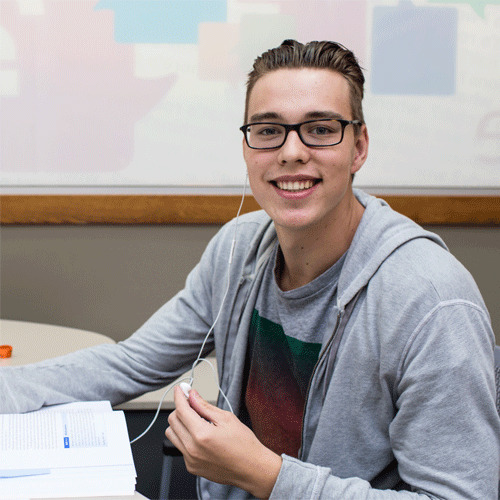
\includegraphics[width=0.4\textwidth]{kevin2.jpg}
\end{wrapfigure}
\textbf{\large Kevin Donnavan (23)} \\ \\
\textbf{Job Title: }Engineering Student\\
\textbf{Education:} 3rd Year Mechanical Engineering\\
\textbf{Experience:}
\begin{compactitem}
\item 3rd Year Mechanical Engineering
\item Summer internship as a junior structural engineer
\item Army reserves - Infantry
\end{compactitem}
\textbf{Skills:}
\begin{compactitem}
\item Problem Solving, Mathematics
\item Programming in Java, C\#, and C++
\end{compactitem}
\textbf{Goals:}
\begin{compactitem}
\item Obtain a good GPA and find a job in his field.
\end{compactitem}
\bigskip 
\textbf{Goals and Tasks user accomplishes}\\
Kevin says he just wants to get through his classes and get a decent GPA. Like everyone, his hardest classes mostly have to do with math (although he feels he is better than average). Kevin will be happy with anything that can make his math calculations easier.\\ \\
\textbf{Problem calculator solves} \\
The calculator helps Kevin get fast answers to difficult math problems he sees in class. Without a calculator, he is not sure how he would calculate the various functions that he sees on a daily basis. The calculator has to be precise enough so he can get the right answer to complex solutions of differential equations but he is not willing to wait - calculation must be near-instantaneous.
\pagebreak


\begin{wrapfigure}{R}{0.4\textwidth}
\includegraphics[width=0.4\textwidth]{tarek2.jpg}
\end{wrapfigure}
\textbf{\large Tarek Ghamzi (23)} \\ \\
\textbf{Job Title: }Engineering Student\\
\textbf{Job Title: }3rd year Electrical engineering student\\
\textbf{Education:} High School + CEGEP, currently in Electrical Engineering\\
\textbf{Experience:}
\begin{compactitem}
\item Subway
\item Pharmacist assistant
\end{compactitem}
\textbf{Skills:}
\begin{compactitem}
\item Problem Solving, Mathematics
\item Programming in C++ , and arduino 
\end{compactitem}
\textbf{Goals:}
\begin{compactitem}
\item Finish his degree with a good GPA
\item Find a job in his field
\end{compactitem}
\bigskip 
\textbf{Goals and Tasks user accomplishes}\\
Tarek claims that his main priority in life at the moment is to get his degree in Electrical Engineering. He claims that his field is heavily based on math, which he struggles with.
He aims to graduate with a higher than average GPA to gain an edge over others in his highly competitive field.\\ \\
\textbf{Problem calculator solves} \\
His calculator helps him in computing the high level mathematical functions that would take hours to solve by himself. It also helps him double check his answers for simple calculations.
Tarek claims that his calculator is with him at all times. Its accuracy, speed and comfort are of highest value to him.

\vspace{0.25in}

\begin{wrapfigure}{R}{0.40\textwidth}

\includegraphics[width=0.40\textwidth]{arash.jpg}
\end{wrapfigure}
\textbf{\Large Arash Mohajer (28)} \\ \\
\textbf{Job Title: }2nd year Avionics Engineering student \\
\textbf{Education:} High School + CEGEP, currently in University\\
\textbf{Experience:}
\begin{compactitem}
\item Completed two internships at a company that manufactures Flight Simulators
\item Worked part time as a waiter
\end{compactitem}
\textbf{Skills:}
\begin{compactitem}
\item Mathematics, Physics
\item Technical Writing
\item Some experience programming in C\# and Java
\end{compactitem}
\textbf{Goals:}
\begin{compactitem}
\item Find more internships during his degree
\item Finish his degree in a reasonable amount of time
\item Save money for his future (manage personal finance)
\end{compactitem}
\bigskip
\textbf{Goals and Tasks user accomplishes}\\
Arash wants to finish his degree in Avionics as soon as possible so that he can get a good job in a field that he enjoys. He wants to continue taking part in engineering competitions and hackathons to learn more about his field and others and to meet other like-minded individuals. He wants to manage his personal finance in order to pay off the debt that he currently has from his university tuition. \\ \\
\textbf{Problem calculator solves}
While he is more focused on graduating than getting good grades in his classes, he has many math and physics intensive classes where he relies on a calculator. He uses a calculator at school for homework, projects and exams. He also uses a calculator for conversion between different units for engineering and physics problems. At home, he uses his calculator to manage his personal finances and to plan his future spending. 
\pagebreak

\begin{wrapfigure}{R}{0.40\textwidth}
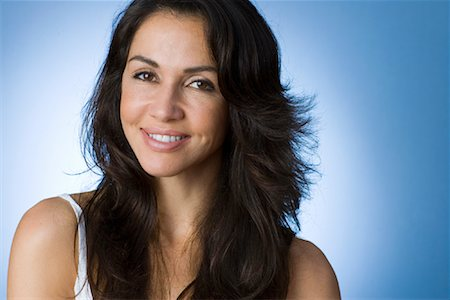
\includegraphics[width=0.40\textwidth]{victoria.jpg}
\end{wrapfigure}
\textbf{\Large Victoria Benlolo (35)} \\ \\
\textbf{Job Title: }1st year HR student\\
\textbf{Education:} High School + CEGEP\\
\textbf{Experience:}
\begin{compactitem}
\item Has owned and managed a spa for 2 years
\item Worked as a financial analyst for 7 years
\end{compactitem}
\textbf{Skills:}
\begin{compactitem}
\itemsep0em 
\item Economics, Business, Finance
\item Public Speaking
\item Investing
\end{compactitem}
\textbf{Goals:}
\begin{compactitem}
\itemsep0em 
\item Maximize the profit of her business
\item Invest in new profitable endeavours 
\item She is interested in opening new spas around town once her business grows more
\item Hire new employees and continue to manage the finances of her business
\end{compactitem}
\bigskip 
\textbf{Goals and Tasks user accomplishes}\\
Victoria wants to continue to grow her business and potentially start franchising her spa to open up new locations around the city. She wants to hire new talent in order to expand her finance team. Her day-to-day includes managing employees' pay, keeping inventory of products, paying bills and managing business income. Additionally, she wants to continue investing in the stock market. \\ \\
\textbf{Problem calculator solves}
At the Spa, Victoria uses a calculator to calculate all of her business expenses, profit/loss, employee salaries, etc. A reliable calculator is very important to her. She uses a calculator to plan expenses in her future business expansion plans.  She also uses a calculator to keep track of how her personal accounts and investment portfolios are growing. 
\pagebreak

\subsection{Appendix D - Use Case Descriptions}

\begin{table}[!h]
\begin{tabular}{|p{3cm}|p{9cm}|}
\hline
\textbf{ID} & UC 1  \\ \hline
\textbf{Name} & Calculate result  \\ \hline
\textbf{Description} & User wants the calculator to resolve his mathematical expression to a satisfactory level of precision near-instantaneously.  \\ \hline
\textbf{Pre-condition} &
	\begin{itemize}
		\vspace{-2mm}
		\item Calculator is on
		\vspace{-3.5mm}
	\end{itemize}  \\ \hline
\textbf{Post-condition} &
	\begin{itemize}
		\vspace{-2mm}
		\item Calculator takes user input, parses, calculates, and arrives at a correct result.
		\item Calculator saves the result of this operation for future use (UC 2).
		\vspace{-3.5mm}
	\end{itemize}  \\ \hline
\textbf{Basic path} &
	\begin{enumerate}
		\vspace{-2mm}
		\item This use case starts with the user entering a mathematical expression into the calculator.
		\item When satisfied with inputted expression user presses "=" button or "enter" on keyboard.
		\item Calculator performs resolution of the arithmetic expression.
		\item Calculator stores the result of the expression (UC 4).
		\vspace{-3.5mm}
	\end{enumerate}  \\ \hline
\textbf{Alternative Path} &
	\begin{itemize}[leftmargin=6mm]
		\vspace{-2mm}
		\item [1b.] User enters a letter and number in order to store a variable (UC 3).
		\item [3a.] Calculator detects a syntax or arithmetic error in user's input.
			\begin{enumerate}
				\item Calculator detect the type of exception.
				\item Calculator displays this exception on screen (UC 4)
				\item User can clear exception and return to the offending arithmetic expression and attempt to correct the error (return to Basic Path 2).
			\end{enumerate}
		
		\vspace{-3.5mm}
	\end{itemize}  \\ \hline
\end{tabular}
\caption{UC 1 - Calculate result}
\end{table}
\pagebreak

\begin{table}[!h]
\begin{tabular}{|p{3cm}|p{9cm}|}
\hline
\textbf{ID} & UC 2  \\ \hline
\textbf{Name} & Recover previous result  \\ \hline
\textbf{Description} & User wants to recall the result of a previous calculation and be able use it in another calculation.  \\ \hline
\textbf{Pre-condition} &
	\begin{itemize}
		\vspace{-2mm}
		\item Calculator is on
		\item A successful calculation has already taken place (UC 1)
		\vspace{-3.5mm}
	\end{itemize}  \\ \hline
\textbf{Post-condition} &
	\begin{itemize}
		\vspace{-2mm}
		\item User sees result of previous calculation and can input it into another calculation.
		\vspace{-3.5mm}
	\end{itemize}  \\ \hline
\textbf{Basic path} &
	\begin{enumerate}
		\vspace{-2mm}
		\item User presses "Ans" button which will input result of the previous calculation into the current calculation.
		\item User carries on with the rest of the calculation (UC 1).
		\vspace{-3.5mm}
	\end{enumerate}  \\ \hline
\textbf{Alternative Path} &
	\begin{itemize}[leftmargin=6mm]
		\vspace{-2mm}
		\item [1a.] User can press "mem" button and see a list of previous results that can be chosen for the current calculation.
			\begin{enumerate}
				\item User presses "mem" button
				\item User scrolls to the desired result
				\item User presses "enter" button to insert select result into current calculation.
			\end{enumerate}
		
		\vspace{-3.5mm}
	\end{itemize}  \\ \hline
\end{tabular}
\caption{UC 2 - Recover previous result}
\end{table}
\pagebreak

\begin{table}[!h]
\begin{tabular}{|p{3cm}|p{9cm}|}
\hline
\textbf{ID} & UC 3  \\ \hline
\textbf{Name} & Store variables  \\ \hline
\textbf{Description} & User want to store values that can be recalled during calculations by referencing an alphabetical label.  \\ \hline
\textbf{Pre-condition} &
	\begin{itemize}
		\vspace{-2mm}
		\item Calculator is on
		\vspace{-3.5mm}
	\end{itemize}  \\ \hline
\textbf{Post-condition} &
	\begin{itemize}
		\vspace{-2mm}
		\item A number is stored in the calculator's memory and is ready to be retrieved by invoking its alphabetical label.
		\item User should be able to clear or overwrite a stored variable.
		\vspace{-3.5mm}
	\end{itemize}  \\ \hline
\textbf{Basic path} &
	\begin{enumerate}
		\vspace{-2mm}
		\item This use case starts with the user entering an alphabetical label that will eventually be used to recall the stored value.
		\item The user then presses "equals" to indicate that a value is to be stored under the chosen label.
		\item The user then presses "enter" which tells the calculator to store the variable under the aforementioned label.
		\item At any point during a calculation (UC 1), the user can evoke the value stored in a variable by entering the corresponding alphabetic character.
		\item The calculator substitutes the variables's value into the calculation.
		\vspace{-3.5mm}
	\end{enumerate}  \\ \hline
\textbf{Alternative Path} &
	\begin{itemize}[leftmargin=6mm]
		\vspace{-2mm}
		\item [1a.] Clearing the variable
			\begin{enumerate}
				\item User enters the alphabetic label of the variable that requires clearing (value and label appear on display).
				\item User presses "clear".
				\item The calculator shows the variable is now cleared.
			\end{enumerate}
		\vspace{-3.5mm}
	\end{itemize}  \\ \hline
\end{tabular}
\caption{UC 3 - Store variables}
\end{table}
\pagebreak

\begin{table}[!h]
\begin{tabular}{|p{3cm}|p{9cm}|}
\hline
\textbf{ID} & UC 4  \\ \hline
\textbf{Name} & Display Result  \\ \hline
\textbf{Description} & User wants clear display of the calculation as it is being inputted. User also wants the calculator to display clear results and appropriate error messages. \\ \hline
\textbf{Pre-condition} &
	\begin{itemize}
		\vspace{-2mm}
		\item Result was calculated, or
		\item User inputs values in calculator
		\vspace{-3.5mm}
	\end{itemize}  \\ \hline
\textbf{Post-condition} & 
	\begin{itemize}
		\vspace{-2mm}
		\item Intermediate calculation is displayed on screen.
		\item Final results are displayed on screen.
		\item Error messages are displayes correctly.
		\vspace{-3.5mm}
	\end{itemize}  \\ \hline
\textbf{Basic path} &
	\begin{enumerate}
		\vspace{-2mm}
		\item User turns on the calculator
			\begin{itemize}
			\item [1a.] Welcome message is displayed.
			\end{itemize}
		\item User enters a calculation. The input calculation is displayed on scree as it is typed.
		\item User presses "=" to calculate (UC 1).
		\item The result of the calculation is displayed on screen.
		\vspace{-3.5mm}
	\end{enumerate}  \\ \hline
\textbf{Alternative Path} &
	\begin{itemize}[leftmargin=6mm]
		\vspace{-2mm}
		\item [4a.] An error occured and the appropriate message is displayed to the user.
			\begin{itemize}
			\item [1] User can clear the error and attempt to correct it.
			\end{itemize}
		
		\vspace{-3.5mm}
	\end{itemize}  \\ \hline
\end{tabular}
\caption{UC 4 - Calculate result}
\end{table}

\pagebreak

\section{F - Draft Calculator User Manual}

\begin{flushleft}

\textbf{\Large Calculator Instructions:}

\begin{enumerate}
\item Start the calculator program 
\item Read the available functions listed
\item Each function will have the number of required parameters in the brackets 
\item type in the function name, along with the function parameters, all seperated by space.
\item type exit to quite the program
\end{enumerate}


\textbf{\Large Function Manual}

Addition (...)
\begin{compactitem}
  \item [] SYNTAX: addition [Double ...]
  \item [] PARAMETER LIMIT: infinite
  \item [] RETURN TYPE: Double
\end{compactitem}
\medskip

Subtraction (...)
\begin{compactitem}
  \item [] SYNTAX: subtraction [Double ...]
  \item [] PARAMETER LIMIT: infinite
  \item [] RETURN TYPE: Double
\end{compactitem}
\medskip

Multiplication (...)
\begin{compactitem}
  \item [] SYNTAX: multiplication [Double ...]
  \item [] PARAMETER LIMIT: infinite
  \item [] DESCRIPTION: Multiplies the all the numbers in the parameters list
  \item [] RETURN TYPE: Double
\end{compactitem}
\medskip

Division (...)
\begin{compactitem}
  \item [] SYNTAX: division [Double ...]
  \item [] PARAMETER LIMIT: infinite
  \item [] RETURN TYPE: Double
  \item [] DESCRIPTION: Divides the first parameters by the 2nd. The answers of 
               that division is divided by the 3rd, which is then 
	       devided by the 4th...
  \item [] RETURN TYPE: Double
\end{compactitem}
\medskip

root (2)
\begin{compactitem}
  \item [] SYNTAX: root [Double] [Integer]
  \item [] PARAMETER LIMIT: 2
  \item [] DESCRIPTION: Calculates the nth root of the 1st parameter, where n is
               the 2nd parameter
  \item [] RETURN TYPE: Double
\end{compactitem}
\medskip

factorial (1)
\begin{compactitem}
  \item [] SYNTAX: factorial [Long/Integer]
  \item [] PARAMETER LIMIT: 1
  \item [] DESCRIPTION: Calculates factorial of the 1st parameter
  \item [] RETURN TYPE: Long
\end{compactitem}
\medskip

ln (1)
\begin{compactitem}
  \item [] SYNTAX: ln [Double]
  \item [] PARAMETER LIMIT: 1
  \item [] DESCRIPTION: Calculates natural logarithm of the 1st parameter
  \item [] RETURN TYPE: Double
\end{compactitem}
\medskip

$e^x$ (1)
\begin{compactitem}
  \item [] SYNTAX: $e^[Double]$
  \item [] PARAMETER LIMIT: 1
  \item [] DESCRIPTION: Calculates Eulers number to the power of 1st parameter
  \item [] RETURN TYPE: Double
\end{compactitem}
\medskip

power (2)
\begin{compactitem}
  \item [] SYNTAX: power [Double, Double]
  \item [] PARAMETER LIMIT: 2
  \item [] DESCRIPTION: Calculates parameter 1 to the power of parameter 2
  \item [] RETURN TYPE: Double
\end{compactitem}
\medskip

\end{flushleft}

\clearpage
\glsaddallunused
\printnoidxglossaries


\end{document}

